\documentclass[12pt,a4paper]{article}
\usepackage{ctex}
\usepackage{amsmath,amscd,amsbsy,amssymb,latexsym,url,bm,amsthm}
\usepackage{epsfig,graphicx,subfigure}
\usepackage{enumitem,balance}
\usepackage{wrapfig}
\usepackage{mathrsfs,euscript}
\usepackage[usenames]{xcolor}
\usepackage{hyperref}
\usepackage[vlined,ruled,linesnumbered]{algorithm2e}
\hypersetup{colorlinks=true,linkcolor=black}

\newtheorem{theorem}{Theorem}
\newtheorem{lemma}[theorem]{Lemma}
\newtheorem{proposition}[theorem]{Proposition}
\newtheorem{corollary}[theorem]{Corollary}
\newtheorem{exercise}{Exercise}
\newtheorem*{solution}{Solution}
\newtheorem{definition}{Definition}
\theoremstyle{definition}

\renewcommand{\thefootnote}{\fnsymbol{footnote}}

\newcommand{\postscript}[2]
 {\setlength{\epsfxsize}{#2\hsize}
  \centerline{\epsfbox{#1}}}

\renewcommand{\baselinestretch}{1.0}

\setlength{\oddsidemargin}{-0.365in}
\setlength{\evensidemargin}{-0.365in}
\setlength{\topmargin}{-0.3in}
\setlength{\headheight}{0in}
\setlength{\headsep}{0in}
\setlength{\textheight}{10.1in}
\setlength{\textwidth}{7in}
\makeatletter \renewenvironment{proof}[1][Proof] {\par\pushQED{\qed}\normalfont\topsep6\p@\@plus6\p@\relax\trivlist\item[\hskip\labelsep\bfseries#1\@addpunct{.}]\ignorespaces}{\popQED\endtrivlist\@endpefalse} \makeatother
\makeatletter
\renewenvironment{solution}[1][Solution] {\par\pushQED{\qed}\normalfont\topsep6\p@\@plus6\p@\relax\trivlist\item[\hskip\labelsep\bfseries#1\@addpunct{.}]\ignorespaces}{\popQED\endtrivlist\@endpefalse} \makeatother

\begin{document}

\noindent

%========================================================================
\noindent\framebox[\linewidth]{\shortstack[c]{
\Large{\textbf{Lab08-Graph Exploration}}\vspace{1mm}\\
CS214-Algorithm and Complexity, Xiaofeng Gao, Spring 2020.}}
\begin{center}
\footnotesize{\color{red}$*$ If there is any problem, please contact TA Yiming Liu.}

% Please write down your name, student id and email.
\footnotesize{\color{blue}$*$ Name:Hanzhang Yang  \quad Student ID:518030910022 \quad Email: linqinluli@sjtu.edu.cn}
\end{center}

\begin{enumerate}
    \item
    \textbf{BFS Tree.} Similar to DFS, BFS yields a tree, (also possibly forest, but \textbf{just consider a tree} in this question) and we can define \textbf{tree, forward, back, cross} edges for BFS. Denote $Dist(u)$ as the distance between node $u$ and the source node in the BFS tree. Please prove:
    \begin{enumerate}
    	\item For both undirected and directed graphs, no forward edges exist in the graph.
    	
    	\item There are no back edges in undirected graph, while in directed graph each back edge $(u,v)$ yields $0\leq Dist(v)\leq Dist(u)$.
    	
    	\item For undirected graph, each cross edge $(u,v)$ yields $Dist(v)=Dist(u)$ or $Dist(v)=Dist(u)+1$, while for directed graph, each cross edge $(u,v)$ yields $Dist(v)\leq Dist(u)+1$.
    	
    \end{enumerate}

	\textbf{Proof.}

	(a) By contradiction. We assume there exists a forward edge. And node $i$ is the ancestor, $j$ is the descendant.

	If the forward edge exists, when building the BFS tree, $j$ must be the child of $i$. Thus there will be a circle which contains the edge $(i,j)$that it's contrary to it's a tree.
	
	Therefore no forward edges exist in the graph.

	(b) By contradiction. Assume there exists a back edge $(u,v)$

	\textbf{Undiredted graphs:}

	For it's a undirected graph, when building BFS tree, $u$ will be the child of $v$. Thus it's contrary to that $(u,v)$ is a back edge.

	Therefore, there  are  no  back  edges  in  undirected  graph.

	\textbf{Directed graphs:}

	If $Dist(v)> Dist(u)$, $v$ will be the descendant of $u$. Thus when building BFS tree, $v$ will be searched earlier than $u$ and $u$ will be the child of $v$, whih is contrary to that $(u,v)$ is a back edge.
	
	Therefore, in  directed  graph  each  back  edge$(u, v)$ yields $ 0\le Dist(v)\le Dist(u)$.

	(c)

	When building BFS tree, every $Dist()$ yields a level. And the search order is according to  the number of $Dist()$.

	\textbf{Undiredted graphs:}

	By contradiction. Assume $|Dist(v)-Dist(u)|\ge 2$.
	
	When building the level according to $min\{ Dist(u),Dist(v)\}+1$. For there exists edge $(u,v)$, $u$ and $v$ will be parent and child. Thus it's contrary to that $(u,v)$ is a cross edge and $|Dist(v)-Dist(u)|=1$.
	
	\textbf{Directed graphs:}

	By contradiction. Assume $Dist(v)-Dist(u)\ge 2$.

	The same as before, When building the level according to $min\{ Dist(u),Dist(v)\}+1$, $v$ hasn't been added another node except $u$. For there exists edge $(u,v)$, $u$ will be the parent of $v$ which causes the contradiction.


	\item 
    \textbf{Articulation Points, Bridges, and Biconnected Components.} Let $G=(V, E)$ be a connected, undirected graph. An articulation point of $G$ is a vertex whose removal disconnects $G$. A bridge of $G$ is an edge whose removal disconnects $G .$ A biconnected component of $G$ is a maximal set of edges such that any two edges in the set lie on a common simple cycle. Figure\ref{def} illustrates these definitions. We can determine articulation points, bridges, and biconnected components using depth-first search. Let $G_{\pi}=\left(V, E_{\pi}\right)$ be a depth-first tree of $G$. Please prove:
    
    \begin{enumerate}
    	\item The root of $G_{\pi}$ is an articulation point of $G$ if and only if it has at least two children in $G_{\pi}$.
    	\item An edge of $G$ is a bridge if and only if it does not lie on any simple cycle of $G$.
    	\item The biconnected components of $G$ partition the nonbridge edges of $G$.
    \end{enumerate}

	 \begin{figure}[htbp]
	 	
		\centering
		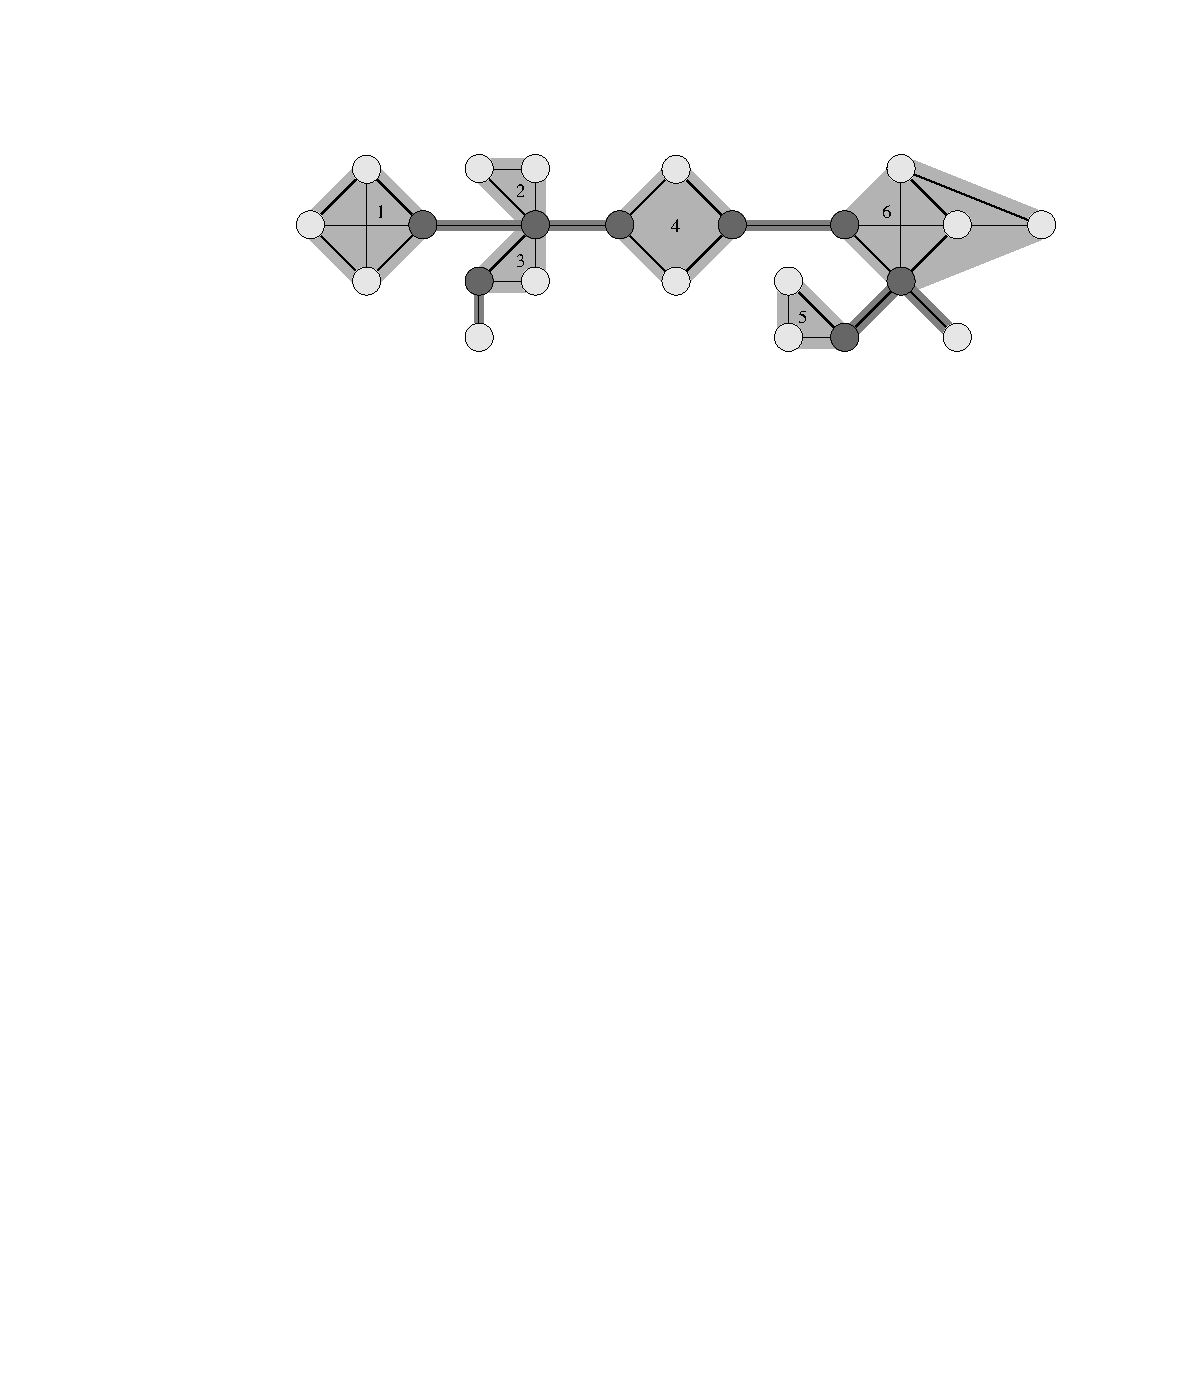
\includegraphics[width=6in]{Fig-Definition.pdf}
		\caption{The definition of articulation points, bridges, and biconnected components. The articulation points are the heavily shaded vertices, the bridges are the heavily shaded edges, and the biconnected components are the edges in the shaded regions, with a \textit{bcc} numbering shown.}
		\label{def}
	\end{figure}

	\textbf{Proof.}
	
	(a)

	\textbf{Necessity.}
	
	For $G_{\pi}$ is a tree, assume the root of $G_{\pi}$ has at least two children.
	After removing the root, its child trees will be disconnected. Thus the root is an articulation point.


	\textbf{Sufficiency.}

	If $G_{\pi}$ is an articulation point of $G$, its removal disconnects $G$. If it has only one child, its removal only causes $G$ become a node and another $tree$.
	Therefore, it has at least two children.

	(b)

	\textbf{Necessity.}

	If an edge does not lie on any simple cycle of $G$, the nodes according to the edge cannot be connected after removing the edge. Thus the whole graph $G$ disconnects too.
	Therefore, the edge is a bridge.

	\textbf{Sufficiency.}

	Assume an edge lies on a simple cycle of $G$. After removing the edge, the circle still connects and $G$ doesn't disconnect too.
	Thus it cannot lie on any simple cycle of $G$.

	(c)
	Consider a biconnected component of $G$. For $G$ is connected graph, the component must connect with at least one edge. 
	Because a biconnected component of $G$ is the maximal set of edges such that any two edges in the set lie on a common simple cycle. 
	The connected edge cannot be added to the biconnected component and it does not lie on any simple cycle. If it lies, it will be in a biconnected component.
	Thus according to (b), the edge is an bridge. And for all edges, it can be either nonbridge or an edge in a biconnected component.

	Therefore, the biconnected components of $G$ partition the nonbridge edges of $G$.
	\item
    Suppose $G=(V, E)$ is a \textbf{Directed Acyclic Graph} (DAG) with positive weights $w(u, v)$ on each edge. Let $s$ be a vertex of $G$ with no incoming edges and assume that every other node is reachable from $s$ through some path.
    
    \begin{enumerate}
    	\item
    	Give an $O(|V|+|E|)$-time algorithm to compute the shortest paths from $s$ to all the other vertices in $G$. Note that this is faster than Dijkstra's algorithm in general.
    	\item
    	Give an efficient algorithm to compute the longest paths from $s$ to all the other vertices.
    \end{enumerate}
	
	\textbf{Solution.}

	For it's a DAG, we can use Dynamic Programming to solve this problem.

	(a)
	We can define $dp[i]$ stores the shortest path weight from node s to i.
	\begin{equation}
		dp(i)=
		\begin{cases}
			0&\mbox{if i=s}\\
			min\{dp(j)+weight(j,i)\}(for\ all\ j\rightarrow i) &\mbox{else}
		\end{cases}
	\end{equation}

	However it needs topologically sort and store all the node in the dp array, which enables the prvious node been visited before the current node.

	Here is the pseudo code 

	\begin{algorithm}[H]
		\KwIn{$G=(V,E)$ and the weights $W(i,j)$}
		\KwOut{the shortest paths weights of all nodes}
		\BlankLine
		\caption{shortest path in DAG}
		$dp[n] = \{0\}$\;
		$node[n] $\;
		$node[1] = s$\;
		topologically sort and store nodes in node[ ]\;
		
		\For{$i=2$ to $n$}{
			$dp[node[i]]=min\{dp[node[j]]+w(j,i)\}$(for all $node[j]\rightarrow node[i]$)
		}
	\end{algorithm}
	
	The time complexity consists of topologically sort which costs $O(|V|+|E|)$ and the traversal which costs $O(|V|+|E|)$.

	Therefore the time complexity is $O(|V|+|E|)$.

	\newpage
	(b)
	We can define $dp[i]$ stores the longest path weight from node $i$ to other nodes.
	\begin{equation}
		dp(i)=
		\begin{cases}
			0&\mbox{if node i's out degree is 0}\\
			max\{dp[j]+weight(i,j)\}\mbox{(for all $i\rightarrow j$)}&else
		\end{cases}
	\end{equation}

	\begin{algorithm}[H]
		\KwIn{$G=(V,E)$ and the weights $W(i,j)$}
		\KwOut{the longest paths weights}
		\BlankLine
		\caption{longest path in DAG}
		$dp[n] = \{0\}$\;
		$node[n] $\;
		$node[1] = s$\;
		topologically sort and store nodes in node[ ]\;
		
		\For{$i=n$ to $1$}{
			\uIf{node i's out degree is 0}{
				$dp[node[i]]=0$\;
			}
			\Else{
				$dp[node[i]]=max\{dp[node[j]+w(i,j)]$\}\mbox{(for all $node[i]\rightarrow node[j]$)}\;
			}
		}
		\textbf{Output} $dp[node[1]]$\;
	\end{algorithm}
	The result is stored in $dp[node[1]]$.
	The time complexity is the same as before which is $O(|V|+|E|)$.



\end{enumerate}

\vspace{20pt}

\textbf{Remark:} You need to include your .pdf and .tex files in your uploaded .rar or .zip file.

%========================================================================
\end{document}
